%%%%%%%%%%%%%%%%%%%%%%%%%%%%%%%%%%%%
% Configuración general de página
%%%%%%%%%%%%%%%%%%%%%%%%%%%%%%%%%%%%
\documentclass[10pt,a4paper]{article}
\textheight = 21cm
\textwidth = 15cm
\topmargin = -0.5 cm
\oddsidemargin = 1cm

%%%%%%%%%%%%%%%%%%%%%%%%%%%%%%%%%%%%
% Paquetes
%%%%%%%%%%%%%%%%%%%%%%%%%%%%%%%%%%%%
\usepackage{amsmath}
\usepackage[utf8]{inputenx} % Permite introducir caracteres no ASCII
\usepackage[spanish]{babel} % Hace que los títulos aparezcan en español
\usepackage[pdftex]{graphicx} % uso de graficos en general
\usepackage{subcaption} % poder poner dos graficos como parte de uno
\usepackage{fancyhdr} % encabezado diferente para pag pares e impares
\usepackage{enumerate} % Permite crear listas
\usepackage{adjustbox}
\usepackage{tabu}
\usepackage{multicol} % Permite combinar columnas
\usepackage{multirow} % Permite combinar filas
\usepackage{colortbl} % Colorear celdas
\usepackage{booktabs} % Bordes en tablas
\usepackage{float} % Tablas y figuras flotantes
\usepackage[tablename=Tabla]{caption} % Permite insertar pies de figuras y títulos de tabla
\usepackage{booktabs}
\usepackage{etoolbox} % Permite arreglar errores de ciertos comandos
\usepackage[svgnames, table]{xcolor} % Colores a usar
\usepackage{footnote} % Notas al pie
\makesavenoteenv{tabular} % Permite insertar notas al pie en tablas
\usepackage[colorlinks=true, linkcolor=black, citecolor=black, urlcolor=cyan]{hyperref} % Permite insertar hyperlinks
\usepackage{url} % Corrige errores causados por la presencia de \, _ y otros caracteres en URLs

%%%%%%%%%%%%%%%%%%%%%%%%%%%%%%%%%%%%
% Configuración del formato del doc.
%%%%%%%%%%%%%%%%%%%%%%%%%%%%%%%%%%%%
\patchcmd{\thebibliography}{\section*{\refname}}{}{}{} % Inserta las referencias sin título
\apptocmd{\sloppy}{\hbadness 10000\relax}{}{} % Evita un warning molesto en la bibliografía
\captionsetup{hypcap=false} % Corrige un warning molesto al utilizar hyperref
\AtBeginDocument{
  \let\oldref\ref
  \def\ref{\oldref*}} % Evita la creación de links en donde se llame al comando \ref
\graphicspath{{figuras/}} % Ubicación de los gráficos
\newcommand{\HRule}{\rule{\linewidth}{0.5mm}}
\DeclareGraphicsExtensions{.png,.jpg,.jpeg} % extensiones de las imágenes
\setlength{\parindent}{0.25in}

%%%%%%%%%%%%%%%%%%%%%%%%%%%%%%%%%%%%
% Incluimos el contenido
%%%%%%%%%%%%%%%%%%%%%%%%%%%%%%%%%%%%
\begin{document}

% Title
\begin{center}


\includegraphics[scale=0.1]{itba_logo}
\vspace{1cm}

\textsc{\LARGE Instrumentación Biomédica II - 16.18}\\[0.2cm]
\textsc{\Large Instituto Tecnológico de Buenos Aires}\\[0.2cm]
\vspace{1cm}

\HRule \\[0.2cm]
{ \huge \bfseries Entrega Final - TP Cuatrimestral \\[0.2cm] }
{ \huge \bfseries Grupo n° 6 \\[0.2cm] }
{ \huge \bfseries \textit{Computarized Auditory Brainstem Response Audiometry} (CABRA) \\[0.2cm] }
\HRule \\[1cm]

\vspace{1cm}

\begin{tabular}{| l | c |}
    \hline
    Presentación & \makebox[2cm]{} \\ \hline
    Desarrollo & \makebox[2cm]{} \\ \hline
    Conclusiones & \makebox[2cm]{} \\ \hline
    Nota Final & \makebox[2cm]{} \\ \hline \hline
    Firma y Fecha & \makebox[2cm]{} \\
    \hline
\end{tabular}

\vspace{1cm}
\begin{multicols}{2}

% Author and supervisor
%\large
\begin{tabular}{l l}
  \emph{PRM}  &  Gustavo Panza \\
  \emph{ATP}  &  Ramón Igarreta \\
  \emph{ATP}  &  Franco Perez Rivera \\
  \emph{Ayudante}  &  Bianca Soto Acosta \\

\end{tabular}


% Integrantes
\columnbreak

%\normalsize
\begin{tabular}{l l}
  \emph{Alumnos:}   &  Lucas Franzi \\ &  Gonzalo Grau \\
                    &  Josué Laszeski \\
\end{tabular}

\end{multicols}
\vspace{1cm}

\textbf{Fecha de entrega}: 17/12/2024

\end{center}


%%%%%%%%%%%%%%%%%%%%%%%%%%%%%%%%%%%%%%%%
%                ENCABEZADO
%%%%%%%%%%%%%%%%%%%%%%%%%%%%%%%%%%%%%%%%
\thispagestyle{empty}
\pagestyle{fancy}
\headheight=60pt 	%para cambiar el tamaño del encabezado
\fancyhead[L]{I.B. II - 16.18 - 2024 2C}
% \fancyhead[C]{
\includegraphics[width=20mm]{itba_logo}}
\fancyhead[C]{\textbf{ITBA}}
\fancyhead[R]{Informe CABRA}

\newpage
\tableofcontents
\newpage
\section{Introducción} \label{introduccion}

La audiometría es un estudio médico realizado con el objetico de evaluar la integridad funcional del sistema auditivo.
La audiometría tonal, en particuarl, es una prueba que se realiza para determinar la capacidad de una persona para escuchar sonidos a diferentes frecuencias y volúmenes.
El objetivo de este estudio es obtener un audiograma, el cual representa los límites audibles (expresados en [dbHL], decibelios normalizados por normoacusia) del paciente para distintos valores de frecuencia de sonido.
La audiometría tonal se realiza en ambos oídos, para determinar la capacidad auditiva de cada oído por separado.
El audiómetro es un dispositivo que genera tonos puros a diferentes frecuencias y volúmenes, reproducidos a través de auriculares \textit{over-ear} que se colocan en la cabeza del paciente y que permiten escuchar los tonos generados.
Mediante un barrido de amplitudes y frecuencias, se obtiene el audiograma del paciente analizando en qué condiciones se percibe y se deja de percibir el estímulo.
Generalmente, es el paciente quien debe indicar si escucha o no los tonos generados por el audiómetro.
Sin embargo, en pacientes que no pueden comunicarse verbalmente, como los bebés, se deben considerar otras técnicas para obtener el audiograma.

El potencial evocado auditivo del tronco cerebral (ABR, por sus siglas en inglés) es una técnica que permite evaluar la integridad de las vías auditivas desde el oído interno hasta el tronco cerebral.
El ABR es un potencial eléctrico generado por la actividad de las neuronas del nervio auditivo y del tronco cerebral en respuesta a un estímulo acústico.
Mediante el análisis de su morfología, detectando latencia y amplitud de ondas tipificadas, es posible detectar la percepción sonora.
Además, se puede evaluar la integridad de las vías auditivas y determinar la presencia de patologías en el sistema auditivo, mediante la obtención de potenciales evocados en respuesta a estímulos transmitidos por vía aérea o por vía ósea.
Esta es una técnica no invasiva, que no requiere la colaboración del paciente y que puede ser utilizada en pacientes de cualquier edad, incluyendo recién nacidos.

CABRA \textit{(Computarized Auditory Brainstem Response Audiometry)} es un sistema de audiometría automática que utiliza la técnica de ABR para obtener el audiograma del paciente.
El sistema CABRA se basa en la generación de estímulos sonoros a través de auriculares (de conducción aérea u ósea), y la medición de la respuesta del sistema auditivo a través de electrodos colocados en la cabeza del paciente.
El objetivo de este sistema es obtener el audiograma del paciente de manera automática, sin necesidad de la colaboración del paciente.
El siguiente manual describe el funcionamiento del sistema CABRA, detallando los pasos necesarios para realizar una audiometría automática y obtener el audiograma en forma semiautomatizada.
\section{Configuración inicial} \label{configuracion}
\subsection{Componentes} \label{componentes}
El dispositivo CABRA cuenta con una parte de hardware y una parte de software.
Su hardware está compuesto por:
\begin{itemize}
    \item Placa de adquisición de datos.
    \item Auriculares de conducción aérea.
    \item Auriculares de conducción ósea.
    \item Electrodos de superficie.
    \item Cable de conexión USB.
    \item Cable de conexión de electrodos.
    \item Carcasa de protección.
\end{itemize}

El software de CABRA es un programa de computadora que se debe instalar en una computadora con sistema operativo Windows 7 o superior.
Se debe contar además con un puerto USB disponible para conectar la placa de adquisición de datos.

\subsection{Instalación del software} \label{instalacion}

Para instalar el software de CABRA, se debe seguir los siguientes pasos:
\begin{enumerate}
    \item Descargar el instalador del software de CABRA desde el siguiente enlace: \url{https://www.cabra.com.ar}.
    \item Ejecutar el instalador y seguir las instrucciones que aparecen en pantalla.
    \item Conectar la placa de adquisición de datos a un puerto USB de la computadora.
    \item Abrir el software de CABRA.
\end{enumerate}

\subsection{Configuración de la placa de adquisición de datos} \label{configuracion_placa}

El primer paso para la configuración de la placa de adquisición es la correcta colocación de los electrodos.
Como se muestra en la Figura \ref{fig:electrodos}, los electrodos deben colocarse en la cabeza del paciente de la siguiente manera:
\begin{itemize}
    \item Electrodo de activo ($V_{in}^{+}$): en la frente del paciente.
    \item Electrodo de tierra ($V_{in}^{-}$): en la apófisis mastoides ipsilateral del paciente.
    \item Electrodo de referencia (neutro): en la apófisis mastoides contralateral del paciente.
\end{itemize}

\begin{figure}[H]
    \centering
    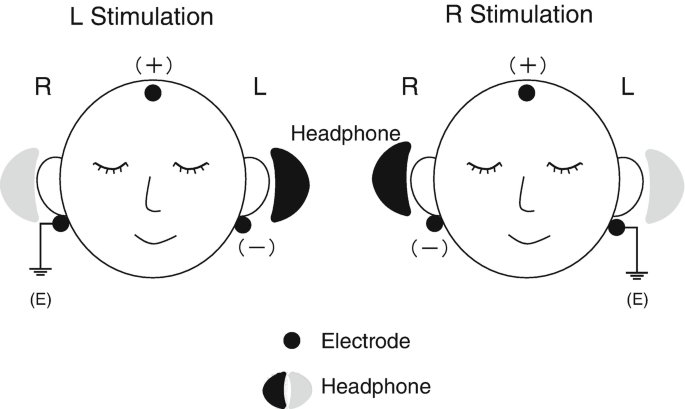
\includegraphics[width=0.5\textwidth]{figuras/electrodos.png}
    \caption{Colocación de los electrodos en la cabeza del paciente, para mediciones de ABR en oido izquierdo (L) o derecho (R).}
    \label{fig:electrodos}
\end{figure}

Luego, encastrar el pin metálico de los electrodos a la ficha hembra de los cables de adquisición.
Finalmente, conectar los cables de adquisición a la placa de adquisición de datos, mediante la entrada auxiliar.
\textit{Observación}: Para evaluar un oído luego de haber evaluado el contraleteral, no desconectar los electrodos
ya colocados.
Simplemente, desencastar los electrodos de la ficha hembra de los cables de adquisición y conectar los electrodos del otro oído.

\subsection{Configuración de los auriculares} \label{configuracion_auriculares}

Los auricuales, sean de conducción ósea o aérea, deben ir conectados a la computadora.
Es vital que se setee el volumen al máximo para realizar las pruebas.
Evitar confusiones de lado para los auriculares, verificando que el canal izquierdo se conecte al oido izquierdo y
viceversa.
\section{Uso de la interfaz gráfica]} \label{GUI}

La interfaz gráfica de usuario (GUI) es la parte del programa que interactúa con el usuario.
Al ejecutar el programa, se abre una ventana que permite al usuario interactuar con el sistema CABRA.
La GUI se divide en cuatri secciones principales:
\begin{itemize}
    \item La barra de tareas, que permite configurar la conexión con el audiometro y especificar parámetros del
    estímulo.
    \item El panel de control, que permite al usuario configurar los parámetros de la audiometría.
    \item El panel de resultados, que muestra los resultados de la audiometría.
    \item La etiqueta de estado, que muestra el estado actual del sistema.
\end{itemize}

\begin{figure}[H]
    \centering
    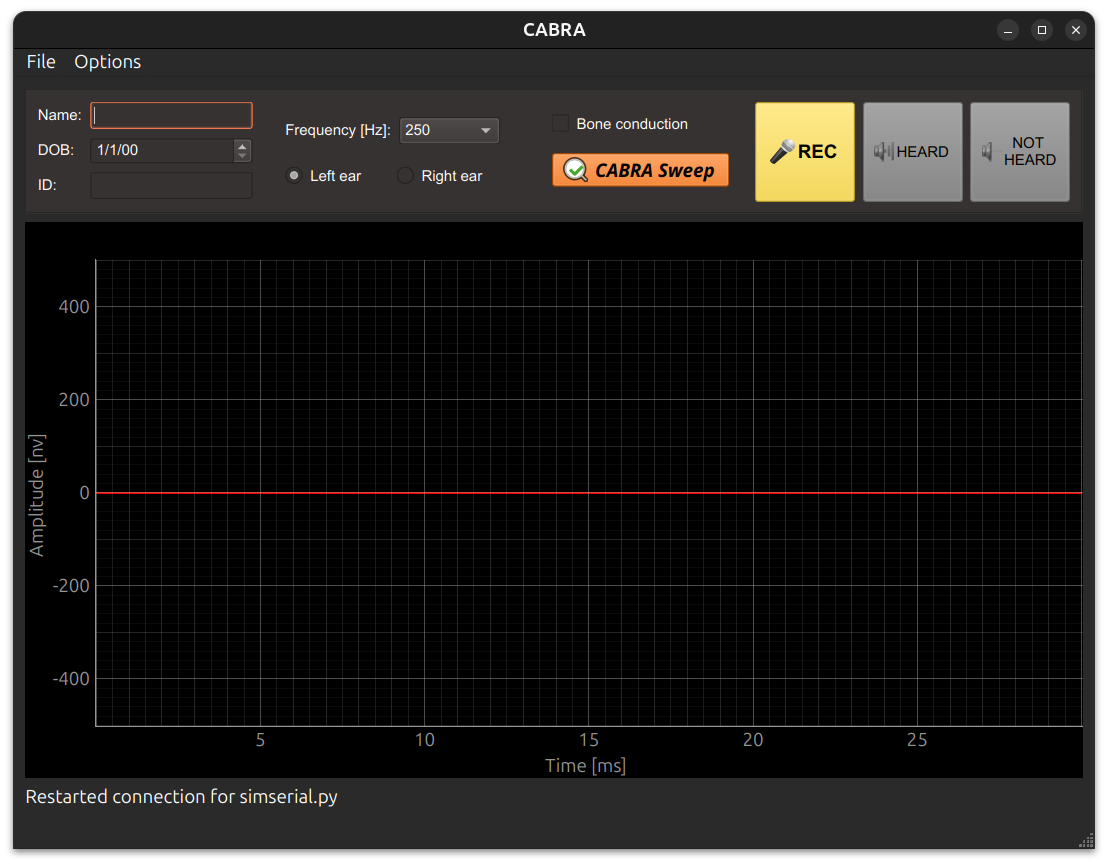
\includegraphics[width=0.8\textwidth]{figuras/gui_basic.png}
    \caption{Interfaz gráfica de usuario de CABRA}
    \label{fig:GUI_basic}
\end{figure}

Durante todo momento, se debe prestar particular atención a la etiqueta de estado, ya que informa al usuario sobre
el estado actual del sistema y sobre los próximos pasos a seguir.

\subsection{Verificación de la conexión con CABRA}

Al inicializar el programa, debería visualizarse en la etiqueta de estado el mensaje \textit{Connection established}.
Caso contrario, se abrirá una ventana emergente que indicando el error.

\begin{figure}[H]
    \centering
    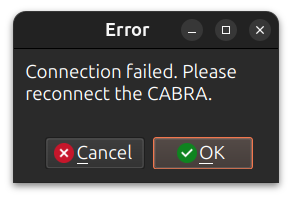
\includegraphics[width=0.4\textwidth]{figuras/connection_error_popup}
    \caption{Ventana emergente de error}
    \label{fig:GUI_conn_error}
\end{figure}

En caso de que se presente un error, se debe verificar que el audiometro esté conectado al puerto USB de la computadora.
Luego, indicar "OK" en la ventana emergente para cerrarla y volver a intentar la conexión.

\textit{Observación}: si se selecciona la opción "Cancel", la ventana emergente se cerrará, y el programa pasará
automáticamente a funcionar en modo de simulación.
La sección \ref{simulacion} describe el modo de simulación en detalle.

\subsection{Realización del estudio de audiometría}

Para realizar la audiometría, se deben configurar algunos parámetros de la prueba.
Estos parámetros se dividen en dos secciones: la información personal del paciente (nombre, fecha de nacimiento,
ID) y la configuración de la audiometría (selección de oído, selección de frecuencia, método de conducción).
Luego, existen dos maneras de llevar a cabo el estudio: forma manual y forma automática.
A continuación, se describen ambas formas.

\subsubsection{Forma manual} \label{manual}

La metodología manual de la audiometría consiste en seleccionar manualmente cada frecuencia y cada oído, indicando
el método de conducción utilizado.
Luego de haber configurado los parámetros, se debe presionar el botón "REC" para comenzar la prueba.
Al oprimir este botón, el programa reproducirá un estímulo auditivo según la configuración seleccionada, a una
amplitud inicial de 0 [dbHL]. Al finalizar el estímulo, se visualizará en pantalla el potencial evocado obtenido,
junto con la onda V detectada.
Entonces, se activarán los botones de "HEARD" y "NOT HEARD", para que el usuario indique si el paciente escuchó o no
el estímulo.
Prestando atención a la etiqueta de estado, notará que el sistema le indicará una sugerencia de diagnóstico:
mediante un algoritmo de análisis de señales, CABRA le indicará si la onda visualizada indica o no percepción sonora.
El usuario no está obligado a seguir esta sugerencia, pero se recomienda hacerlo en casos de duda.

Al indicar si el sonido fue perceptible o no, mediante los ya mencionados botones de "HEARD" y "NOT HEARD", CABRA
automáticamente generará un nuevo estímulo auditivo, con una amplitud mayor o menor, según corresponda.
Este proceso se repetirá hasta que se encuentra, automáticamente, el umbral auditivo del paciente.
En ese momento, se visualizará en pantalla en la etiqueta de estado el valor de dicho umbral.
Este valor quedará almacenado internamente, y se utilizará más adelante para visualizar el audiograma.


\begin{figure}[H]
    \centering
    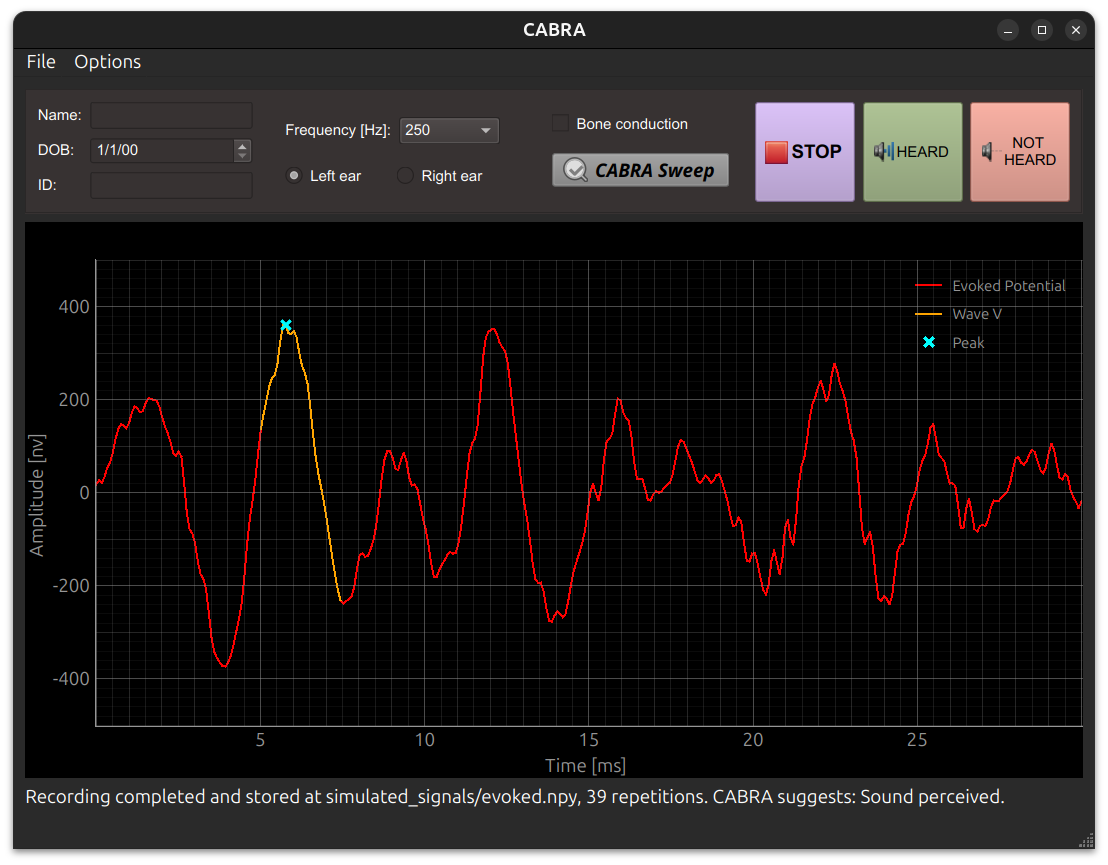
\includegraphics[width=0.8\textwidth]{figuras/cabra_gui_test_evoked}
    \caption{Interfaz gráfica de usuario de CABRA durante la realización de una audiometría}
    \label{fig:GUI_manual}
\end{figure}

Para continuar con el estudio, se debe realizar un barrido completo de todas las frecuencias y ambos oídos.
Al finalizar, se visualizará en pantalla el audiograma del paciente, y se almacenará en un archivo.

\begin{figure}[H]
    \centering
    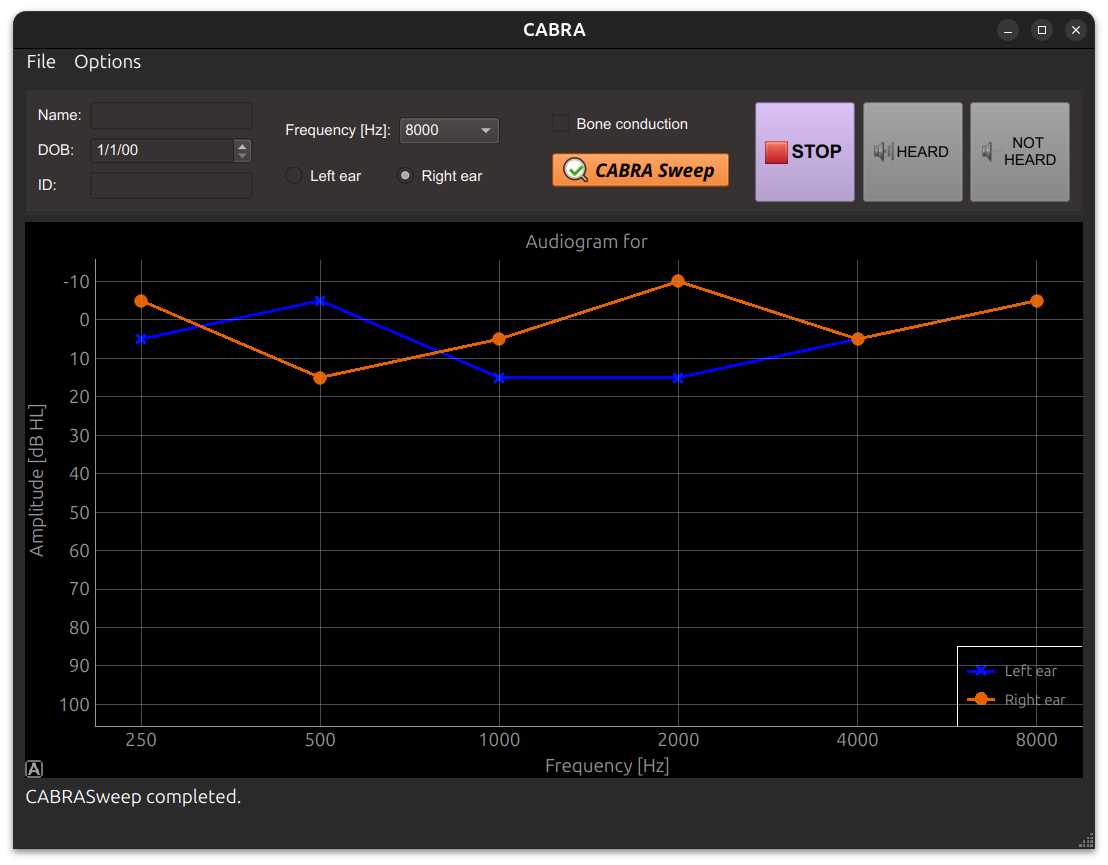
\includegraphics[width=0.8\textwidth]{figuras/GUI_audiogram}
    \caption{Interfaz gráfica de usuario de CABRA al finalizar una audiometría}
    \label{fig:GUI_audiogram}
\end{figure}


\subsubsection{Forma automática (CABRASweep)}

Realizar un barrido manual de todo el rando de frecuencias para ambos oídos puede ser tedioso y llevar mucho tiempo.
Además, es posible que el usuario cometa errores al seleccionar los parámetros, como ignorar una prueba o evaluar
dos veces las mismas condiciones.
Para evitar esto, CABRA cuenta con el botón \textit{CABRASweep}, que permite realizar un barrido automático de todas
las frecuencias y ambos oídos.
Al presionar este botón, el programa realizará automáticamente todas las pruebas, avanzando de frecuencia en
frecuencia.
El usuario, por su parte, sólo deberá indicar si el paciente escuchó o no cada estímulo, de la misma manera que se
describió en la sección anterior.%  \ref{manual}.
%Al finalizar, se visualizará en pantalla el audiograma del paciente, y se almacenará en un archivo.






\section{Archivos} \label{archivos}

El sistema CABRA almacena los resultados de las audiometrías en archivos binarios, además de guardar las
audiometrías.
Los potenciales evocados se guardan en la carpeta \textit{saved\_data}, nomenclados según el siguiente formato:

\begin{center}
    \textit{frecuencia\_ID\_fecha\_hora.npz}
\end{center}

Con respecto a los audiogramas, estos se guardarán en la carpeta \textit{saved\_audiometries}, con el formato

\begin{center}
    \textit{ID\_fecha\_hora.png}
\end{center}


\section{Conclusión} \label{conclusion}

Para cualquier consulta con respecto a la operación del sistema CABRA, no dude en contactar a los desarrolladores:

\begin{itemize}
    \item \textbf{Lucas Franzi} - \
    \href{mailto:lfranzi@itba.edu.ar}{lfranzi@itba.edu.ar}
    \item \textbf{Gonzalo Grau} - \
    \href{mailto:ggrau@itba.edu.ar}{ggrau@itba.edu.ar}
    \item \textbf{Josué Laszeski} - \
    \href{mailto:jlaszeski@itba.edu.ar}{jlaszeski@itba.edu.ar}
\end{itemize}


\end{document}